\documentclass[journal,onecolumn]{IEEEtran}

% , - Packages , , , , , , , , , , , , , , , , , , , -
\usepackage[utf8]{inputenc}
\usepackage[T1]{fontenc}
\usepackage{textcomp}
\usepackage{amsmath,amssymb,amsfonts}
\usepackage{graphicx}
\usepackage{subfig}
\usepackage{bm}
\usepackage{url}
\usepackage{xcolor}
\usepackage[colorlinks=true,allcolors=blue]{hyperref}

% , - Convenience macros , , , , , , , , , , , , , , , , -
\newcommand{\Tris}{T-RIS}
\newcommand{\Rris}{R-RIS}
\DeclareMathOperator*{\argmax}{arg\,max}

\usepackage{xr}
\externaldocument{RIS_MFSK_TVT}
\renewcommand{\thefigure}{S\arabic{figure}}
\renewcommand{\thetable}{S\arabic{table}}
\graphicspath{{figures/}}
\begin{document}
\title{Supplementary Material for ``A Two-Stage Reconfigurable Intelligent Surface\\
Architecture for Decoupled M-FSK Modulation and\\
Beamforming in 28-GHz Bistatic Sensing''}
\maketitle
Equation, figure and table numbers without the prefix S refer to the main paper.

\begin{figure}[!h]
\centering
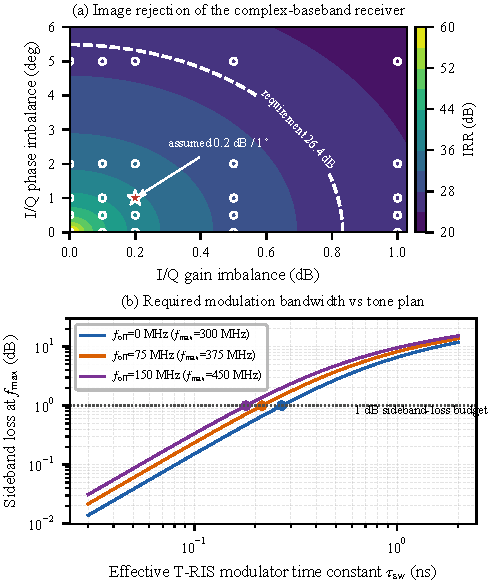
\includegraphics[width=0.9\columnwidth]{FC_sideband_separation}
\caption{(a) Image-rejection ratio \eqref{eq:irr} versus I/Q gain and phase imbalance; circles are time-domain correlator simulations, the dashed contour is the 26.4\,dB requirement and the star the assumed imbalance. (b) Sideband loss at the highest tone versus the effective \Tris{} modulator time constant for three tone plans; dots mark the 1\,dB limit.}
\label{fig:sideband}
\end{figure}

\clearpage
\begin{table}[!h]
\centering
\caption{Tone-plan options: RF guard band versus required T-RIS modulation bandwidth}
\label{tab:tone_plan}
\footnotesize
\setlength{\tabcolsep}{1.8pt}
\begin{tabular}{@{}ccccccc@{}}
\hline\hline
$f_{\mathrm{off}}$ & Tones & Image guard & $\tau_{\mathrm{sw}}^{\max}$ & Max squint & $\Delta R_{\mathrm{path}}$ & $\sqrt{\mathrm{CRB}_L}$ \\
(MHz) & (MHz) & (MHz) & (ns) & (deg, \% HPBW) & (m) & (cm) \\
\hline
0 & 25--300 & 50 (0.18\,\%) & 0.27 & 1.04 (8.2\,\%) & 1.00 & 1.87 \\
75 & 100--375 & 200 (0.71\,\%) & 0.22 & 1.29 (10.1\,\%) & 1.00 & 1.87 \\
150 & 175--450 & 350 (1.25\,\%) & 0.18 & 1.53 (12.1\,\%) & 1.00 & 1.87 \\
\hline\hline
\multicolumn{7}{@{}p{0.95\columnwidth}@{}}{\scriptsize $\tau_{\mathrm{sw}}^{\max}$: largest effective modulator time constant keeping the sideband loss at $f_{\max}$ within 1\,dB. Squint at $\theta_1=60^\circ$. Resolution and CRB are independent of $f_{\mathrm{off}}$; operating point $\mathrm{SNR}_1=-14.5$\,dB.}
\end{tabular}
\end{table}

\clearpage
\begin{table}[!h]
\centering
\caption{Multi-Tone Beam Coherence of the Two-Stage R-RIS ($N_x=16$, $M=12$, $f_{m,M}=300$\,MHz)}
\label{tab:squint}
\footnotesize
\setlength{\tabcolsep}{1.6pt}
\begin{tabular}{@{}cccccccc@{}}
\hline\hline
$\theta_1$ & Design & HPBW & Max squint & Worst & Aggr. & CRB & Bias \\
(deg) & freq. & (deg) & (deg, \% HPBW) & (dB) & (dB) & (+\%) & (mm) \\
\hline
30 & $f_c$ & 7.3 & 0.35 (4.8) & 0.026 & 0.010 & 0.13 & 0.00 \\
30 & centre & 7.3 & 0.16 (2.2) & 0.005 & 0.002 & 0.04 & 0.00 \\
60 & $f_c$ & 12.7 & 1.04 (8.2) & 0.079 & 0.029 & 0.40 & 0.00 \\
60 & centre & 12.7 & 0.49 (3.9) & 0.016 & 0.006 & 0.13 & 0.00 \\
75 & $f_c$ & 24.5 & 2.12 (8.7) & 0.098 & 0.037 & 0.50 & 0.00 \\
75 & centre & 24.5 & 1.09 (4.4) & 0.021 & 0.008 & 0.17 & 0.00 \\
\hline\hline
\multicolumn{8}{@{}p{0.97\columnwidth}@{}}{\scriptsize Worst/Aggr.: loss toward the target of the worst tone and of the mean tone power, relative to the design frequency. CRB: increase of \eqref{eq:crb_R} from the tone-dependent gains. Bias: noise-free bias of the ML path estimate. A single-stage STM-RIS re-steered per symbol has zero squint but reloads $M$ phase maps per sweep.}
\end{tabular}
\end{table}

\clearpage
\begin{table}[!h]
\centering
\caption{Positioning Versus Receive Aperture ($\beta=60^\circ$, Rx--Target Distance 8\,m)}
\label{tab:rx_aperture}
\footnotesize
\setlength{\tabcolsep}{1.5pt}
\begin{tabular}{@{}ccccccccc@{}}
\hline\hline
$N_{\rm rx}$ & $D$ & $G_{\rm rx}$ & $2D^2/\lambda$ & $\sqrt{\mathrm{CRB}_L}$ & $\sqrt{\mathrm{CRB}_\theta}$ & $\sqrt{\mathrm{CRB}_{\rm pos}}$ & RMSE & RMSE \\
 & (cm) & (dBi) & (m) & (cm) & (deg) & (cm) & focused & far field \\
\hline
4 & 1.6 & 12 & 0.0 & 3.74 & 1.1048 & 17.99 & 19.00 & 19.00 \\
8 & 3.7 & 15 & 0.3 & 2.65 & 0.3812 & 6.39 & 6.71 & 6.70 \\
16 & 8.0 & 18 & 1.2 & 1.87 & 0.1340 & 2.49 & 2.46 & 2.46 \\
32 & 16.6 & 21 & 5.1 & 1.32 & 0.0473 & 1.17 & 1.15 & 1.15 \\
64 & 33.7 & 24 & 21.2 & 0.94 & 0.0167 & 0.68 & 0.70 & 0.72 \\
128 & 68.0 & 27 & 86.3 & 0.66 & 0.0059 & 0.45 & 0.45 & 14.31 \\
\hline\hline
\multicolumn{9}{@{}p{0.97\columnwidth}@{}}{\scriptsize Half-wavelength spacing; $G_{\rm rx}$ and $\mathrm{SNR}_1$ scale with $N_{\rm rx}$ from the 16-element values of Table~\ref{tab:sys_params}. RMSE in cm (Monte Carlo); ``focused'' scans with the Rx--target distance known from the path estimate.}
\end{tabular}
\end{table}

\clearpage
\begin{table}[!h]
\centering
\caption{Transmit-Side DC Power Budget, Identical Accounting ($N=256$)}
\label{tab:power_budget}
\footnotesize
\begin{tabular}{@{}lr@{}}
\hline\hline
Item & W \\
\hline
\multicolumn{2}{@{}l}{\emph{Two-stage RIS (PIN, 2 mW/element/layer, $E_{\rm sw}=P_{\rm bias}\tau_{\rm sw}$)}}\\
CW source (PA, 20 %) & 0.500 \\
T-RIS PIN bias & 0.512 \\
R-RIS bias & 0.512 \\
T-RIS switching & 0.045 \\
Controller, DDS, clock & 0.150 \\
\textbf{Total} & \textbf{1.719} \\
\hline
\multicolumn{2}{@{}l}{\emph{AESA, 5\,mW / 15\,mW per channel}}\\
T/R channels & 1.280 \\
LO distribution, main amplifier & 0.870 \\
Controller & 0.150 \\
\textbf{Total (5 / 15 mW)} & \textbf{2.300 / 4.860} \\
\hline
Common bistatic receiver (excluded) & 0.630 \\
\hline\hline
\end{tabular}
\end{table}

\end{document}
